\documentclass{vkr}
\usepackage[english, russian]{babel} % переносы
\usepackage{graphicx} % для вставки картинок
\graphicspath{{images/}} % путь к изображениям
\usepackage[hidelinks]{hyperref}
\usepackage{float} % определяет метод H для рисунка с переносом на следующую страницу, ели не помещается
\usepackage{pdflscape}
\addto{\captionsrussian}{\renewcommand{\refname}{СПИСОК ИСПОЛЬЗОВАННЫХ ИСТОЧНИКОВ}}
\usepackage{xltabular} % для вставки таблиц
\usepackage{makecell}
\renewcommand\theadfont{} % шрифт в /thead
\usepackage{array} % для определения новых типов столбцов таблиц
\newcolumntype{T}{>{\centering\arraybackslash}X} % новый тип столбца T - автоматическая ширина столбца с выравниванием по центру
\newcolumntype{R}{>{\raggedleft\arraybackslash}X} % новый тип столбца R - автоматическая ширина столбца с выравниванием по правому краю
\newcolumntype{C}[1]{>{\centering\let\newline\\\arraybackslash\hspace{0pt}}m{#1}} % новый тип столбца C - фиксированная ширина столбца с выравниванием по центру
\newcolumntype{r}[1]{>{\raggedleft\arraybackslash}p{#1}} % новый тип столбца r - фиксированная ширина столбца с выравниванием по правому краю
\newcommand{\centrow}{\centering\arraybackslash} % командой \centrow можно центрировать одну ячейку (заголовок) в столбце типа X или p, оставив в оcтальных ячейках другой тип выравнивания
\newcommand{\finishhead}{\endhead\hline\endlastfoot}
\newcommand{\continuecaption}[1]{\caption*{#1}\\ \hline }
\usepackage{etoolbox}
\AtBeginEnvironment{xltabular}{\refstepcounter{tablecnt}} % подсчет таблиц xltabular, обычные таблицы подсчитываются в классе

\usepackage[tableposition=top]{caption} % подпись таблицы вверху
\captionsetup{strut=off}
\setlength{\intextsep}{0pt} % Vertical space above & below [h] floats
\setlength{\textfloatsep}{0pt} % Vertical space below (above) [t] ([b]) floats
\DeclareCaptionLabelFormat{gostfigure}{Рисунок #2} %подпись рисунка
\DeclareCaptionLabelFormat{gosttable}{Таблица #2} %подпись таблицы
\DeclareCaptionLabelSeparator{gost}{~--~} %разделитель в рисунках и таблицах
\captionsetup{labelsep=gost}
\captionsetup[figure]{aboveskip=10pt,belowskip=4mm,justification=centering,labelformat=gostfigure} % настройка подписи рисунка
\captionsetup[table]{font={stretch=1.41},skip=0pt,belowskip=0pt,aboveskip=8.5pt,singlelinecheck=off,labelformat=gosttable} % настройка подписи таблицы

\setlength{\LTpre}{8mm} % отступ сверху таблицы
\setlength{\LTpost}{6mm} % отступ снизу таблицы

\usepackage{enumitem}
\setlist{nolistsep,wide=\parindent,itemindent=*} % отступы вокруг списков, выравнивание с учетом разделителя

\usepackage{color} %% это для отображения цвета в коде
\usepackage{listings} %% листинги кода
\setmonofont[Scale=0.7]{Verdana} % моноширный шрифт для листинга

\definecolor{codegreen}{rgb}{0,0.6,0}
\definecolor{codegray}{rgb}{0.5,0.5,0.5}
\definecolor{codepurple}{rgb}{0.58,0,0.82}

\lstset{ %
language=C,                 % выбор языка для подсветки (здесь это С)
numbers=left,               % где поставить нумерацию строк (слева\справа)
numberstyle=\tiny,           % размер шрифта для номеров строк
stepnumber=1,                   % размер шага между двумя номерами строк
numbersep=5pt,                % как далеко отстоят номера строк от подсвечиваемого кода
commentstyle=\color{codegreen},
keywordstyle=\color{magenta},
numberstyle=\tiny\color{codegray},
stringstyle=\color{codepurple},
basicstyle=\linespread{0.95}\ttfamily,
backgroundcolor=\color{white}, % цвет фона подсветки - используем \usepackage{color}
showspaces=false,            % показывать или нет пробелы специальными отступами
showstringspaces=false,      % показывать или нет пробелы в строках
showtabs=false,             % показывать или нет табуляцию в строках
frame=single,              % рисовать рамку вокруг кода
tabsize=2,                 % размер табуляции по умолчанию равен 2 пробелам
captionpos=t,              % позиция заголовка вверху [t] или внизу [b] 
breaklines=true,           % автоматически переносить строки (да\нет)
breakatwhitespace=false, % переносить строки только если есть пробел
escapeinside={\%*}{*)}   % если нужно добавить комментарии в коде
}

\makeatletter % чтобы допускались русские комментарии в листингах
\lst@InputCatcodes
\def\lst@DefEC{%
 \lst@CCECUse \lst@ProcessLetter
  ^^80^^81^^82^^83^^84^^85^^86^^87^^88^^89^^8a^^8b^^8c^^8d^^8e^^8f%
  ^^90^^91^^92^^93^^94^^95^^96^^97^^98^^99^^9a^^9b^^9c^^9d^^9e^^9f%
  ^^a0^^a1^^a2^^a3^^a4^^a5^^a6^^a7^^a8^^a9^^aa^^ab^^ac^^ad^^ae^^af%
  ^^b0^^b1^^b2^^b3^^b4^^b5^^b6^^b7^^b8^^b9^^ba^^bb^^bc^^bd^^be^^bf%
  ^^c0^^c1^^c2^^c3^^c4^^c5^^c6^^c7^^c8^^c9^^ca^^cb^^cc^^cd^^ce^^cf%
  ^^d0^^d1^^d2^^d3^^d4^^d5^^d6^^d7^^d8^^d9^^da^^db^^dc^^dd^^de^^df%
  ^^e0^^e1^^e2^^e3^^e4^^e5^^e6^^e7^^e8^^e9^^ea^^eb^^ec^^ed^^ee^^ef%
  ^^f0^^f1^^f2^^f3^^f4^^f5^^f6^^f7^^f8^^f9^^fa^^fb^^fc^^fd^^fe^^ff%
  ^^^^20ac^^^^0153^^^^0152%
  % Basic Cyrillic alphabet coverage
  ^^^^0410^^^^0411^^^^0412^^^^0413^^^^0414^^^^0415^^^^0416^^^^0417%
  ^^^^0418^^^^0419^^^^041a^^^^041b^^^^041c^^^^041d^^^^041e^^^^041f%
  ^^^^0420^^^^0421^^^^0422^^^^0423^^^^0424^^^^0425^^^^0426^^^^0427%
  ^^^^0428^^^^0429^^^^042a^^^^042b^^^^042c^^^^042d^^^^042e^^^^042f%
  ^^^^0430^^^^0431^^^^0432^^^^0433^^^^0434^^^^0435^^^^0436^^^^0437%
  ^^^^0438^^^^0439^^^^043a^^^^043b^^^^043c^^^^043d^^^^043e^^^^043f%
  ^^^^0440^^^^0441^^^^0442^^^^0443^^^^0444^^^^0445^^^^0446^^^^0447%
  ^^^^0448^^^^0449^^^^044a^^^^044b^^^^044c^^^^044d^^^^044e^^^^044f%
  ^^^^0401^^^^0451%
  %%%
  ^^00}
\lst@RestoreCatcodes
\makeatother


% Режим шаблона (должен быть включен один из трех)
\ВКРtrue
%\Практикаtrue
%\Курсоваяtrue

\newcommand{\Дисциплина}{<<Проектирование и архитектура программных систем>>} % для курсовой
\newcommand{\КодСпециальности}{09.03.04} % Курсовая
\newcommand{\Специальность}{Программная инженерия} % Курсовая
\newcommand{\Тема}{Разработка web-сайта «Русатом – Аддитивные технологии» на платформе} % ВКР Курсовая
\newcommand{\ТемаВтораяСтрока}{1С-Битрикс}
\newcommand{\ГдеПроводитсяПрактика}{Юго-Западном государственном университете} % для практики
\newcommand{\РуководительПрактПредпр}{Куркина А. В.} % для практики
\newcommand{\ДолжнРуководительПрактПредпр}{директор} % для практики
\newcommand{\РуководительПрактУнивер}{Чаплыгин А. А.} % для практики
\newcommand{\ДолжнРуководительПрактУнивер}{к.т.н. доцент} % для практики
\newcommand{\Автор}{И. И. Иванов}
\newcommand{\АвторРод}{Иванова И.И.}
\newcommand{\АвторПолностьюРод}{Иванова Ивана Ивановича} % для практики
\newcommand{\Шифр}{хх-хх-хххх}
\newcommand{\Курс}{4} % для практики
\newcommand{\Группа}{ПО-92б}
\newcommand{\Руководитель}{А. А. Чаплыгин} % для ВКР и курсовой
\newcommand{\Нормоконтроль}{А. А. Чаплыгин} % для ВКР
\newcommand{\ЗавКаф}{А. В. Малышев} % для ВКР
\newcommand{\ДатаПриказа}{«07» апреля 2023~г.} % для ВКР
\newcommand{\НомерПриказа}{1505-с} % для ВКР
\newcommand{\СрокПредоставления}{«13» июня 2023~г.} % для ВКР, курсового

\begin{document}
\maketitle
\ifПрактика{}\else{
   \newpage
\begin{center}
\large\textbf{Минобрнауки России}

\large\textbf{Юго-Западный государственный университет}
\vskip 1em
\normalsize{Кафедра программной инженерии}
\vskip 1em
\ifВКР{
        \begin{flushright}
        \begin{tabular}{p{.4\textwidth}}
        \centrow УТВЕРЖДАЮ: \\
        \centrow Заведующий кафедрой \\
        \hrulefill \\
        \setarstrut{\footnotesize}
        \centrow\footnotesize{(подпись, инициалы, фамилия)}\\
        \restorearstrut
        «\underline{\hspace{1cm}}»
        \underline{\hspace{3cm}}
        20\underline{\hspace{1cm}} г.\\
        \end{tabular}
        \end{flushright}
        }\fi
\end{center}
\vspace{1em}
  \begin{center}
  \large
\ifВКР{
ЗАДАНИЕ НА ВЫПУСКНУЮ КВАЛИФИКАЦИОННУЮ РАБОТУ
  ПО ПРОГРАММЕ БАКАЛАВРИАТА}
  \else
ЗАДАНИЕ НА КУРСОВУЮ РАБОТУ (ПРОЕКТ)
\fi
\normalsize
  \end{center}
\vspace{1em}
{\parindent0pt
  Студента \АвторРод, шифр\ \Шифр, группа \Группа
  
1. Тема «\Тема\ \ТемаВтораяСтрока»
\ifВКР{
утверждена приказом ректора ЮЗГУ от \ДатаПриказа\ № \НомерПриказа
}\fi.

2. Срок предоставления работы к защите \СрокПредоставления

3. Исходные данные для создания программной системы:

3.1. Перечень решаемых задач:}

\renewcommand\labelenumi{\theenumi)}

\begin{enumerate}
\item проанализировать IT-инфраструктуру предприятия;
\item  разработать концептуальную модель системы управления IT-ин\-фра\-струк\-турой предприятия на основе подхода к управлению и организации ИТ-услуг ITSM;
\item спроектировать программную систему управления IT-ин\-фра\-струк\-турой предприятия;
\item сконструировать и протестировать программную систему управления IT-инфраструктурой предприятия.
\end{enumerate}

{\parindent0pt
  3.2. Входные данные и требуемые результаты для программы:}

\begin{enumerate}
\item Входными данными для программной системы являются: данные
справочников комплектующих, конфигураций, ПО, критериев качества SLA,
ИТ-услуг, департаментов компании; технические данные ИТ-ресурсов; данные входящих заявок на ИТ-ресурсы; данные запросов поставщикам на комплектующие.
\item Выходными данными для программной системы являются: сформированные заявки на обслуживание ИТ-ресурсов; сформированные запросы на
закупку комплектующих; сведения о выполненных работах по заявкам; статусы заявок; выходные отчеты (инфографика) – по качеству услуг, по состоянию ИТ-ресурсов, по деятельности ИТ-отдела, по стоимости обслуживания
ИТ-ресурсов, воронка заявок.
\end{enumerate}

{\parindent0pt

  4. Содержание работы (по разделам):
  
  4.1. Введение
  
  4.1. Анализ предметной области
  
4.2. Техническое задание: основание для разработки, назначение разработки,
требования к программной системе, требования к оформлению документации.

4.3. Технический проект: общие сведения о программной системе, проект
данных программной системы, проектирование архитектуры программной системы, проектирование пользовательского интерфейса программной системы.

4.4. Рабочий проект: спецификация компонентов и классов программной системы, тестирование программной системы, сборка компонентов программной системы.

4.5. Заключение

4.6. Список использованных источников

5. Перечень графического материала:

\списокПлакатов

\vskip 2em
\begin{tabular}{p{6.8cm}C{3.8cm}C{4.8cm}}
Руководитель \ifВКР{ВКР}\else работы (проекта) \fi & \lhrulefill{\fill} & \fillcenter\Руководитель\\
\setarstrut{\footnotesize}
& \footnotesize{(подпись, дата)} & \footnotesize{(инициалы, фамилия)}\\
\restorearstrut
Задание принял к исполнению & \lhrulefill{\fill} & \fillcenter\Автор\\
\setarstrut{\footnotesize}
& \footnotesize{(подпись, дата)} & \footnotesize{(инициалы, фамилия)}\\
\restorearstrut
\end{tabular}
}

\renewcommand\labelenumi{\theenumi.}

   \abstract{РЕФЕРАТ}

Объем работы равен \formbytotal{lastpage}{страниц}{е}{ам}{ам}. Работа содержит \formbytotal{figurecnt}{иллюстраци}{ю}{и}{й}, \formbytotal{tablecnt}{таблиц}{у}{ы}{}, \arabic{bibcount} библиографических источников и \formbytotal{числоПлакатов}{лист}{}{а}{ов} графического материала. Количество приложений – 2. Графический материал представлен в приложении А. Фрагменты исходного кода представлены в приложении Б.

Перечень ключевых слов: игра, Система, платформер, 2D, Python, геймплей, дизайн, управление, уровни, классы, подсистема, компонент, модуль, сущность, метод, пользователь.

Объектом разработки является 2D игра платформер.

Целью курсовой работы является создание игры.

В процессе создания сайта были выделены основные сущности, использованы классы и методы модулей, обеспечивающие работу с сущностями предметной области, а также корректную работу игры, разработаны основные аспекты геймплея.


\selectlanguage{english}
\abstract{ABSTRACT}
  
The volume of work is \formbytotal{lastpage}{page}{}{s}{s}. The work contains \formbytotal{figurecnt}{illustration}{}{s}{s}, \formbytotal{tablecnt}{table}{}{s}{s}, \arabic{bibcount} bibliographic sources and \formbytotal{числоПлакатов}{sheet}{}{s}{s} of graphic material. The number of applications is 2. The graphic material is presented in annex A. The layout of the site, including the connection of components, is presented in annex B.

The list of keywords: game, System, platformer, 2D, Python, gameplay, design, management, levels, classes, subsystem, component, module, entity, method, user.

The object of development is a 2D platformer game.

The purpose of the course work is to create a game.

In the process of creating the site, the main entities were identified, classes and methods of modules were used to ensure work with the entities of the subject area, as well as the correct operation of the game, the main aspects of gameplay were developed.
\selectlanguage{russian}
}\fi
\tableofcontents
\section*{ОБОЗНАЧЕНИЯ И СОКРАЩЕНИЯ}

ИС -- информационная система.

КТС -- комплекс технических средств.

ПО -- программное обеспечение.

РП -- рабочий проект.

ТЗ -- техническое задание.

ТП -- технический проект.

UML (Unified Modelling Language) -- язык графического описания для объектного моделирования в области разработки программного обеспечения.

\ifПрактика{}\else{\section*{ВВЕДЕНИЕ}
\addcontentsline{toc}{section}{ВВЕДЕНИЕ}

В мире современных компьютерных технологий разработка компьютерных игр остается одним из наиболее захватывающих и творческих направлений в программировании. В этом контексте, жанр 2D платформеров привлекает внимание разработчиков и геймеров своей простотой, ностальгическим воспоминанием о классических играх и бесконечными возможностями для креативного дизайна.

2D платформеры, наследники золотой эры видеоигр, предоставляют уникальный опыт игрокам, основанный на преодолении препятствий, управлении персонажем в ограниченном двухмерном пространстве и погружении в захватывающие приключения. Этот жанр не только оживляет воспоминания о первых видеоиграх, но и постоянно эволюционирует, внедряя новые технологии и идеи в свой дизайн.

Целью данной курсовой работы является исследование и разработка 2D платформера с использованием современных инструментов и технологий. В процессе работы мы сосредоточим внимание на ключевых аспектах геймдизайна, анимации, управления и создания увлекательных уровней. Кроме того, мы рассмотрим технические аспекты, такие как выбор языка программирования, использование специализированных библиотек и создание интерфейса пользователя.

Эта курсовая работа призвана предоставить комплексный обзор процесса разработки 2D платформера, обогатив тем самым понимание основных принципов геймдизайна и программирования в контексте игр данного жанра. В дальнейшем, результаты данной работы могут служить основой для дальнейших исследований и проектов в области разработки компьютерных игр.

\emph{Цель настоящей работы} – разработка игры платформера и её движка. Для достижения поставленной цели необходимо решить \emph{следующие задачи:}
\begin{itemize}
\item провести анализ предметной области;
\item разработать концептуальную модель игры;
\item спроектировать игру;
\item реализовать игру.
\end{itemize}

\emph{Структура и объем работы.} Отчет состоит из введения, 4 разделов основной части, заключения, списка использованных источников, 2 приложений. Текст выпускной квалификационной работы равен \formbytotal{page}{страниц}{е}{ам}{ам}.

\emph{Во введении} сформулирована цель работы, поставлены задачи разработки, описана структура работы, приведено краткое содержание каждого из разделов.

\emph{В первом разделе} на стадии описания технической характеристики предметной области приводится сбор информации.

\emph{Во втором разделе} на стадии технического задания приводятся требования к разрабатываемой игре.

\emph{В третьем разделе} на стадии технического проектирования представлены проектные решения для игры.

\emph{В четвертом разделе} приводится список классов и их методов, использованных при разработке игры, производится тестирование разработанной игры.

В заключении излагаются основные результаты работы, полученные в ходе разработки.

В приложении А представлен графический материал.
В приложении Б представлены фрагменты исходного кода. 
}\fi
\section{Анализ предметной области}
\subsection{Исследование понятия и история появления жанра платформер}

Жанр компьютерных игр “платформер” (от англ. platform - платформа) зародился в начале 80-х годов прошлого века и стал одним из первых видов видеоигр. Он был создан в результате эволюции аркадных игр, таких как “Space Invaders” и “Pac-Man”, где игрок управлял персонажем на двухмерной плоскости. Платформеры были популярны на игровых автоматах, а затем перешли на домашние компьютеры и игровые консоли.

Платформер - это жанр, в котором игрок управляет персонажем, перемещающимся по платформам и преодолевающим различные препятствия. Главная задача игрока - пройти уровень от начала до конца, собирая различные предметы и избегая опасностей.

Одним из первых представителей жанра считается игра “Donkey Kong” для аркадного автомата Nintendo, выпущенная в 1981 году. В этой игре игрок управлял человеком, пытающимся спасти свою подружку от обезьяны. Персонаж мог прыгать, а также забираться на платформы и ящики. Игра стала очень популярной, и ее успех привел к созданию многих других платформеров на протяжении следующих десятилетий.

В 1982 году компания Nintendo выпустила игру “Mario Bros.”, в которой игрок управлял братом Марио - Луиджи. Эта игра стала основой для многих будущих платформеров, включая серию “Super Mario Bros.”

Ранние платформеры обычно состояли из уровней, где персонаж должен был преодолеть различные препятствия, такие как пропасти, шипы, враги и ловушки, чтобы достичь конца уровня. Некоторые игры также включали элементы головоломки, где игрок должен был использовать предметы или решать задачи, чтобы продвинуться дальше.

С развитием технологий и графики в середине 90-х жанр платформера стал более разнообразным и детализированным. Появились игры с трехмерной графикой, такие как “Crash Bandicoot” и “Spyro the Dragon”, а также игры с элементами паркура, как “Prince of Persia”.

Сегодня платформеры продолжают оставаться популярными, особенно среди детей и подростков. Они часто включают в себя элементы приключений, головоломок и мультиплеера, а также имеют разнообразные сюжетные линии и персонажей. Многие современные игры сочетают элементы платформера с другими жанрами, такими как гонки, шутеры и ролевые игры, создавая новые и интересные игровые опыты.

Жанр платформера продолжает развиваться и адаптироваться к новым технологиям, оставаясь одним из самых популярных и любимых жанров компьютерных игр.
\subsection{Анализ поджанров платформеров}

Жанр платформера включает в себя множество поджанров, каждый из которых имеет свои уникальные особенности и характеристики. Вот некоторые из наиболее распространенных поджанров платформеров:

2D-платформеры: Это классический поджанр платформеров, который включает в себя игры с двухмерной графикой и управлением. Примеры таких игр включают “Super Mario Bros.”, “Kirby’s Epic Yarn” и “Shantae”.

3D-платформеры: Этот поджанр включает в себя платформеры с трехмерной графикой и физикой. Примеры включают “Ratchet and Clank”, “Jak and Daxter” и “Tomb Raider”.

Метроидвания: Это платформеры, которые сочетают в себе элементы метроидвании и платформера. Примеры включают “Castlevania: Symphony of the Night”, “Bloodstained: Ritual of the Night” и “Dead Cells”.

Паркур-платформеры: Эти игры включают в себя элементы паркура и платформера, такие как прыжки, лазание и бег по стенам. Примеры включают серию игр “Mirror’s Edge”, “Assassin’s Creed” и “Prince of Persia”.
\subsection{Анализ существующих разработок}

Среди популярных платформеров можно выделить следующие игры:

Super Mario Bros. - классический 2D платформер, в котором игрок управляет персонажем по имени Марио, преодолевая различные препятствия и сражаясь с врагами.

Kirby’s Epic Yarn - 2D платформер с уникальной графикой и игровым процессом, где игрок управляет персонажем Кирби, способным менять свою форму и использовать различные способности.

Ratchet and Clank - 3D платформер с элементами экшена и головоломок, в котором игроки управляют двумя героями - Рэтчетом и Кланком, сражающимися с различными врагами и решающими загадки.

Castlevania: Symphony of the Night - игра в жанре метроидвания, сочетающая в себе платформер и исследование мира, где игроки управляют вампиром, способным превращаться в различных существ и использовать разное оружие.

Mirror’s Edge - паркур-платформер с видом от первого лица, где игроки могут бегать, прыгать и выполнять различные трюки, преодолевая препятствия и сражаясь с противниками.

Каждая из этих игр имеет свои особенности и уникальный геймплей, который привлекает игроков разных возрастов и предпочтений.

\section{Техническое задание}
\subsection{Основание для разработки}

Основанием для разработки является задание на курсовую работу "<Разработка компьютерной игры в жанре платформер на языке Python">.

\subsection{Цель и назначение разработки}

Основной целью курсовой работы является разработка компьютерной игры в жанре платформер.

Назначение проекта заключается в развлечении потенциального потребителя.

Задачами данной разработки являются:
\begin{itemize}
\item разработка архитектуры приложения;
\item разработка интерфейса приложения;
\item реализация базовой логики и физики игры;
\item создание системы конструктора уровней;
\item обработка событий;
\item реализация отображения игры на экране.
\end{itemize}

\subsection{Требования пользователя к интерфейсу игры}

Игра должна включать в себя:
\begin{itemize}
    \item возможность управления персонажем;
    \item графическое оформление интерфейса;
    \item базовый редактор уровней.
\end{itemize}

Композиция шаблона сайта представлена на рисунке ~\ref{templ:image}.

\begin{figure}[ht]
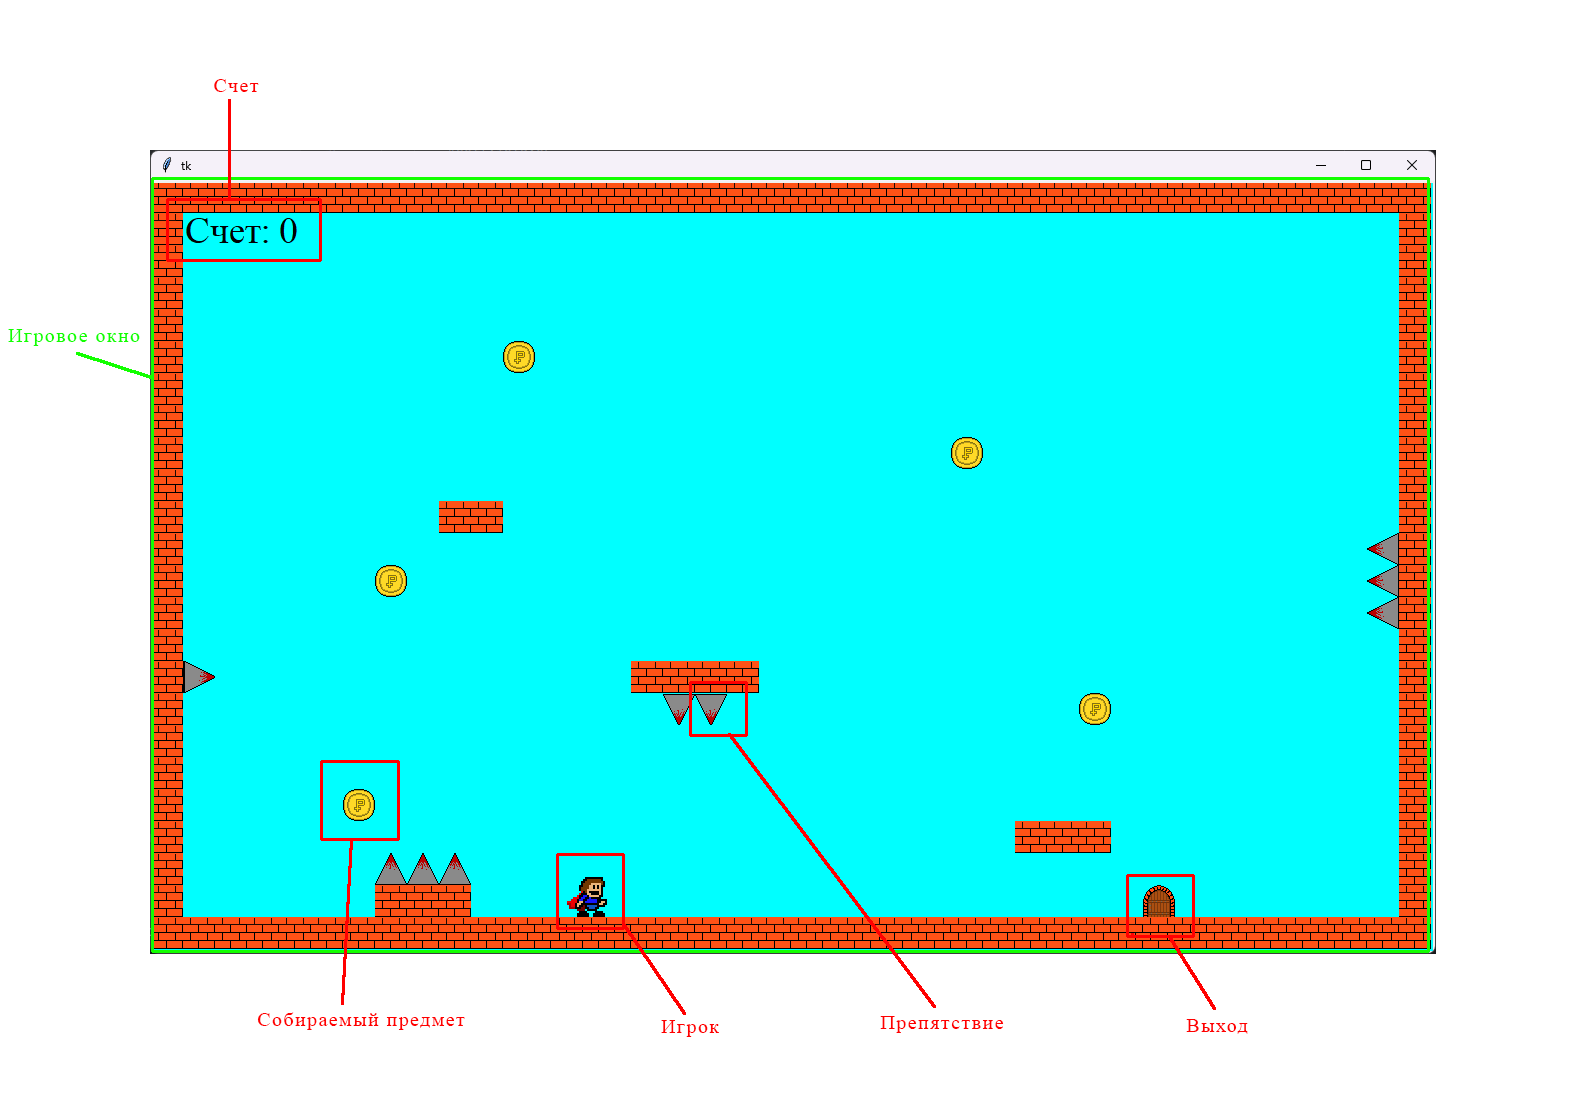
\includegraphics[width=1\linewidth]{templ}
\caption{Композиция шаблона игры}
\label{templ:image}
\end{figure}
%\vspace{-\figureaboveskip} % двойной отступ не нужен (можно использовать, если раздел заканчивается картинкой)

\subsection{Моделирование вариантов использования}

Для разрабатываемой игры была реализована модель, которая обеспечивает наглядное представление вариантов использования.

Она помогает в физической разработке и детальном анализе взаимосвязей объектов. При построении диаграммы вариантов использования применяется унифицированный язык визуального моделирования UML.

Диаграмма вариантов описывает функциональное назначение разрабатываемой системы. То есть это то, что система будет непосредственно делать в процессе своего функционирования. Она является исходным концептуальным представлением системы в процессе ее проектирования и разработки. Проектируемая система представляется в виде ряда прецедентов, предоставляемых системой актерам или сущностям, которые взаимодействуют с системой. Актером или действующим лицом является сущность, взаимодействующая с системой извне (например, человек, техническое устройство). Прецедент служит для описания набора действий, которые система предоставляет актеру.

На основании анализа предметной области в программе должны быть реализованы следующие прецеденты:
\begin{enumerate}
\item Запуск игры.
\item Прохождение уровня.
\item Создание уровня.
\item Отображение окна с результатом.
\end{enumerate}

\subsection{Требования к оформлению документации}

Разработка программной документации и программного изделия должна производиться согласно ГОСТ 19.102-77 и ГОСТ 34.601-90. Единая система программной документации.

\section{Технический проект}
\subsection{Общая характеристика организации решения задачи}

Необходимо спроектировать и разработать игру, которая должна соответствовать всем предъявленным к ней требованиям.

Компьютерная игра — это форма развлечения, предназначенная для запуска и игры на компьютере. Она включает в себя визуальные, звуковые и интерактивные элементы, предоставляя пользователю виртуальное окружение, где тот может взаимодействовать с созданным миром, управлять персонажами и решать различные задачи. Компьютерные игры могут быть разнообразными и включать в себя различные жанры, такие как стратегии, шутеры, головоломки, ролевые игры, платформеры и другие.

\subsection{Обоснование выбора технологии проектирования}

На сегодняшний день информационный рынок, поставляющий программные решения в выбранной сфере, предлагает множество продуктов, позволяющих достигнуть поставленной цели – разработки игры.

\subsubsection{Описание используемых технологий и языков программирования}

В процессе разработки игры используются язык программирования и программные средства, которые применяются для круга задач, при решении которых они необходимы.

\subsubsection{Язык программирования Python}

Питон (Python) - высокоуровневый язык программирования общего назначения с динамической строгой типизацией и автоматическим управлением памятью, ориентированный на повышение производительности разработчика, читаемости кода и его качества, а также на обеспечение переносимости написанных на нём программ.

\paragraph{Достоинства языка Python}

Вот некоторые из основных достоинств Python:

\begin{enumerate}
	\item Простота и читаемость кода:
	
	Python ставит акцент на читаемости кода, что делает его пригодным для быстрого и легкого написания программ. Ясный и понятный синтаксис помогает новичкам и специалистам одинаково.
	\item Интерпретируемость:
	
	Интерпретируемость Python обеспечивает быструю разработку и тестирование кода. Без необходимости компиляции, изменения могут быть внесены и протестированы непосредственно.
	\item Обширная стандартная библиотека:
	
	Python поставляется с обширной стандартной библиотекой, предоставляя разработчикам множество инструментов и модулей для решения разнообразных задач, таких как работа с файлами, сетевое программирование, обработка данных, создание игр и многое другое.
	\item Объектно-ориентированное программирование:
	
	Python поддерживает объектно-ориентированное программирование (ООП), что позволяет создавать модульный и структурированный код, упрощая его повторное использование и сопровождение.
	\item Динамическая типизация:
	
	Динамическая типизация Python позволяет гибко использовать переменные, не требуя их явного объявления типа. Это упрощает написание и изменение кода.
	\item Поддержка сторонних библиотек и фреймворков:
	
	Существует огромное количество сторонних библиотек и фреймворков для Python, таких как Django для веб-разработки, NumPy и Pandas для анализа данных, TensorFlow для машинного обучения, Pygame для игр, что делает его мощным инструментом в различных областях.
	\item Переносимость:
	
	Python является кроссплатформенным, что означает, что программы, написанные на Python, могут быть запущены на различных операционных системах без изменений кода.
\end{enumerate}

\paragraph{Недостатки языка Python}

Хотя Python является мощным и популярным языком программирования, у него также есть некоторые недостатки, которые могут влиять на выбор его использования в конкретных сценариях. Вот несколько из них:

\begin{enumerate}
	\item Производительность:
	
	Python обычно менее эффективен в выполнении определенных задач по сравнению с компилируемыми языками, такими как C++ или Java. Это особенно заметно в вычислительно интенсивных приложениях.
	\item Поддержка мобильной разработки:
	
	Python не является основным языком для мобильной разработки, хотя существуют некоторые фреймворки, такие как Kivy или BeeWare, которые позволяют создавать мобильные приложения на Python. Однако в данном контексте часто предпочитаются другие языки, такие как Java (Android) или Swift (iOS).
	\item Глобальная блокировка интерпретатора (GIL):
	
	GIL в Python представляет собой ограничение, которое позволяет только одному потоку исполнения выполняться в определенный момент времени. Это может стать проблемой в многопроцессорных системах, где несколько ядер могут оставаться неиспользуемыми.
	\item Объем памяти:
	
	Python может потреблять больше памяти по сравнению с некоторыми языками программирования из-за своей динамической природы.
	\item Отсутствие некоторых особенностей в сравнении с компилируемыми языками:
	
	Python может не подходить для разработки низкоуровневых систем или приложений, требующих максимальной производительности и полного контроля над ресурсами
\end{enumerate}

\subsection{Диаграмма компонентов и схема обмена данными между файлами компонента}

Диаграмма компонентов описывает особенности физического представления разрабатываемой игры. Она позволяет определить архитектуру игры, установив зависимости между программными компонентами, в роли которых может выступать как исходный, так и исполняемый код. Основными графическими элементами диаграммы компонентов являются компоненты, интерфейсы, а также зависимости между ними. На рисунке \ref{comp:image} изображена диаграмма компонентов для проектируемой игры. Она включает в себя игровое окно, в котором отображены счет и игровые объекты. Они делятся на собираемые предметы, препятствия, платформы, объект выхода и объект игрока.

\begin{figure}[ht]
\center{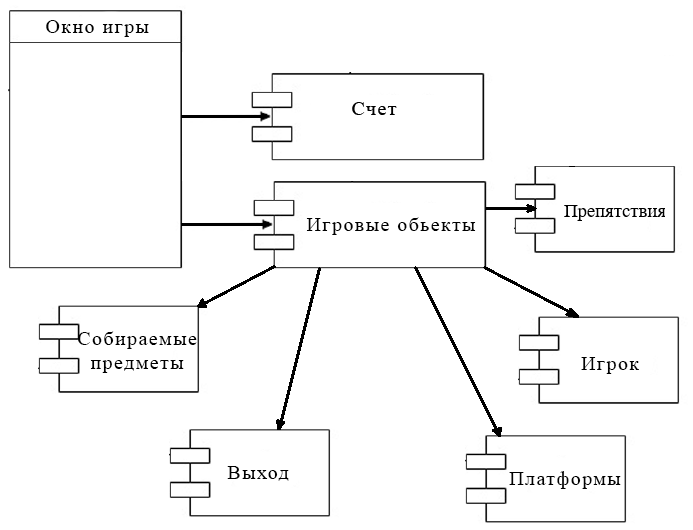
\includegraphics[width=1\linewidth]{comp}}
\caption{Диаграмма компонентов}
\label{comp:image}
\end{figure}

Любой компонент должен быть вызван в сценарии игры. Игра передает данные компоненту в момент вызова последнего.

На рисунке \ref{data:image} представлена схема обмена данными между сценариями игры при взаимодействии компонентов.

\begin{figure}[ht]
\center{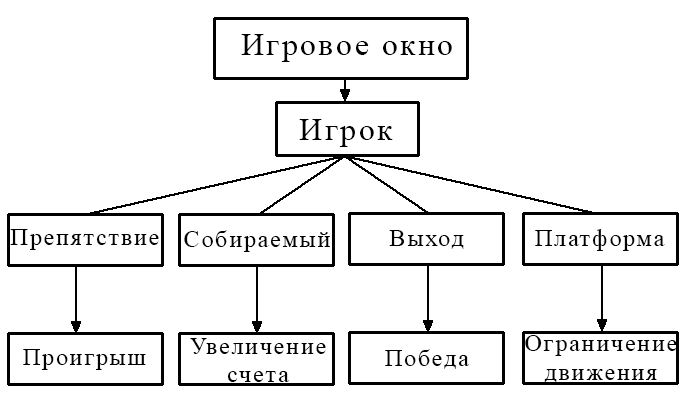
\includegraphics[width=1\linewidth]{data}}
\caption{Диаграмма компонентов}
\label{data:image}
\end{figure}

При взаимодействии с компонентом в сценарии игры происходит распознавание взаимодействующих объектов.

При взаимодействии игрока с разными объектами происходят разные действия. Например при соприкосновении с платформой сбоку игрок не может идти дальше, если платформа находится сверху игрок не может прыгнуть выше и ударяется об нее, если она снижу игрок перестает падать и останавливается на платформе. При соприкосновении игрока с собираемыми предметами, они удаляются с экрана и увеличивают счет. При соприкосновении игрока с препятствие игрок проигрывает. При соприкосновении игрока с выходом, если собраны все предметы, уровень завершается.

Работа компонента заканчивается в момент завершения работы сценария игры или удаления компонента с экрана.

\subsection{Основные сущности игры}

Проанализировав требования, можно выделить две основных сущности:
\begin{itemize}
\item "<Игровой объект">;
\item "<Анимация">.
\end{itemize}

В состав сущности "<Игровой объект"> можно включить атрибуты, представленные в таблице \ref{news:table}.

\begin{xltabular}{\textwidth}{|l|l|p{1.7cm}|X|}
	\caption{Атрибуты сущности "<Игровой объект">\label{news:table}}\\ \hline
	\centrow Поле & \centrow Тип & \centrow Обяза\-тельное & \centrow Описание \\ \hline
	\thead{1} & \thead{2} & \centrow 3 & \centrow 4 \\ \hline
	\endfirsthead
	\thead{1} & \thead{2} & \centrow 3 & \centrow 4 \\ \hline
	\finishhead
	\ id & int & true & Уникальный идентификатор \\ \hline 
	tag & str & true & тег объекта \\ \hline 
	animations & Animation & false & Анимации объекта \\ \hline 
	currentAnim & str & false & Ключ текущей анимации
\end{xltabular}

В состав сущности "<Анимация"> можно включить атрибуты, представленные в таблице \ref{news:table}.

\begin{xltabular}{\textwidth}{|l|l|p{1.7cm}|X|}
	\caption{Атрибуты сущности "<Анимация">\label{news:table}}\\ \hline
	\centrow Поле & \centrow Тип & \centrow Обяза\-тельное & \centrow Описание \\ \hline
	\thead{1} & \thead{2} & \centrow 3 & \centrow 4 \\ \hline
	\endfirsthead
	\thead{1} & \thead{2} & \centrow 3 & \centrow 4 \\ \hline
	\finishhead
	\ frame & int & true & Индекс кадра \\ \hline 
	time & int & true & Скорость анимации \\ \hline 
	name & str & true & Название анимации \\ \hline 
	anim & list[PhotoImage] & true & Список кадров \\ \hline
	n & int & true & Количество кадров \\ \hline
	filename & str & true & Имя файла
\end{xltabular}
\ifПрактика{}\else{
   \section{Рабочий проект}
\subsection{Классы, используемые при разработке сайта}

Можно выделить следующий список классов и их методов, использованных при разработке игры (таблица \ref{class:table}).

\renewcommand{\arraystretch}{0.8} % уменьшение расстояний до сетки таблицы
\begin{xltabular}{\textwidth}{|X|p{2.5cm}|>{\setlength{\baselineskip}{0.7\baselineskip}}p{4.85cm}|>{\setlength{\baselineskip}{0.7\baselineskip}}p{4.85cm}|}
\caption{Описание классов, используемых в приложении\label{class:table}}\\
\hline \centrow \setlength{\baselineskip}{0.7\baselineskip} Название класса & \centrow \setlength{\baselineskip}{0.7\baselineskip} Модуль, к которому относится класс & \centrow Описание класса & \centrow Методы \\
\hline \centrow 1 & \centrow 2 & \centrow 3 & \centrow 4\\ \hline
\endfirsthead
\caption*{Продолжение таблицы \ref{class:table}}\\
\hline \centrow 1 & \centrow 2 & \centrow 3 & \centrow 4\\ \hline
\finishhead
Animation & Модуль графики & Animation – Класс анимации игры. Создает анимации и хранит все информацию о её состоянии & def onTimetAnimation(self) Счетчик кадров анимации

def get\_frame(self) Возвращает текущий кадр

def crop(self) Разбиение на кадры

def rotateImg(self, img, t) Вращение изображения, img : PhotoImage изображение, t : str действие. Возвращает повернутое на 90 или 180 градусов изображение или отзеркаливает его

def makeTransparent(self, img) Прозрачность изображения, img : PhotoImage изображение. Возвращает изображение, удаляя весь белый цвет\\
\hline GameObject & Модуль логики & GameObject – Класс игровых объектов & def change\_anim(self, name) Изменение текущей анимации объекта, name : str ключ анимации

def find\_animation(self, name) Поиск анимации по названию, name : str название анимации. Возвращает анимация с названием\\
\hline Graphics & Модуль графики & Graphics – Класс отображения игрового движка & def change\_frame(self, id, img) Смена кадра анимации, id : int id объекта, sprite : PhotoImage кадр анимации

def add\_anim(self) Добавляет анимацию в словарь

def onTimer(self) Цикл анимаций\\
\hline Game & Модуль логики & Game – Класс игрового движка & def initGame(self) Инициализация всех начальных значений для переменных

def loadImages(self) Загрузка начальных спрайтов

def bind(self, up, left, right) Установка клавиш управления, up : str клавиша прыжка, left : str клавиша движения влево, right : str клавиша движения вправо

def movePlayer(self) Передвижение спрайта игрока

def create\_map(self, level, widht) Создание карты по массиву, level : list[str] массив с ключами, widht : int ширина клетки на карте в пикселях

def add\_gameobjects(self, tag) Добавляет к списку объектов все объекты с тегом, tag : str тег объектов

def find\_objects\_tag(self, tag) Возвращает список объектов с тегом, tag : str тег объектов

def find\_object\_id(self, id) Возвращает объект с соответствующим id, id : int id объекта\\
\hline  &  &  & def checkCollisions(self, anchor) Проверка коллизий игрока, anchor : str направление движения игрока

def checkWallCollision(self, x1, x2, y1, y2, anchor, key) Проверка коллизий со стенами, x1 : int, x2 : int, y1 : int, y2 : int
координаты, anchor : str направление движения игрока, key : str нажатая клавиша

def change\_animation(self, id, name) Изменяет текующую анимацию объекта, id : int id объекта, name : str ключ анимации

def add\_animations(self) Добавление анимаций

def onTimer(self) Игровой цикл\\
\hline MyGame & Главный модуль & Game – Класс игры & def run(self) Запуск mainloop для Tk

def update(self) Обновление игры Запускает основной цикл

def keys(self, keyup, keyleft, keyright) Установка клавиш управления, keyup : str клавиша прыжка, keyleft : str клавиша движения влево, keyright : str клавиша движения вправо

def onKeyPressed(self, e) Вызывается при нажатии клавиш на клавиатуре

def onKeyRelease(self, e) Вызывается при отжатии клавиш на клавиатуре

def drawScore(self) Отрисовка счета

def endGame(self) Выводит сообщение в конце игры

\end{xltabular}
\renewcommand{\arraystretch}{1.0} % восстановление сетки

\subsection{Системное тестирование разработанной игры}

На рисунке \ref{main:image} представлено главное окно игры.
\newpage % при необходимости можно переносить рисунок на новую страницу
\begin{figure}[H] % H - рисунок обязательно здесь, или переносится, оставляя пустоту
\center{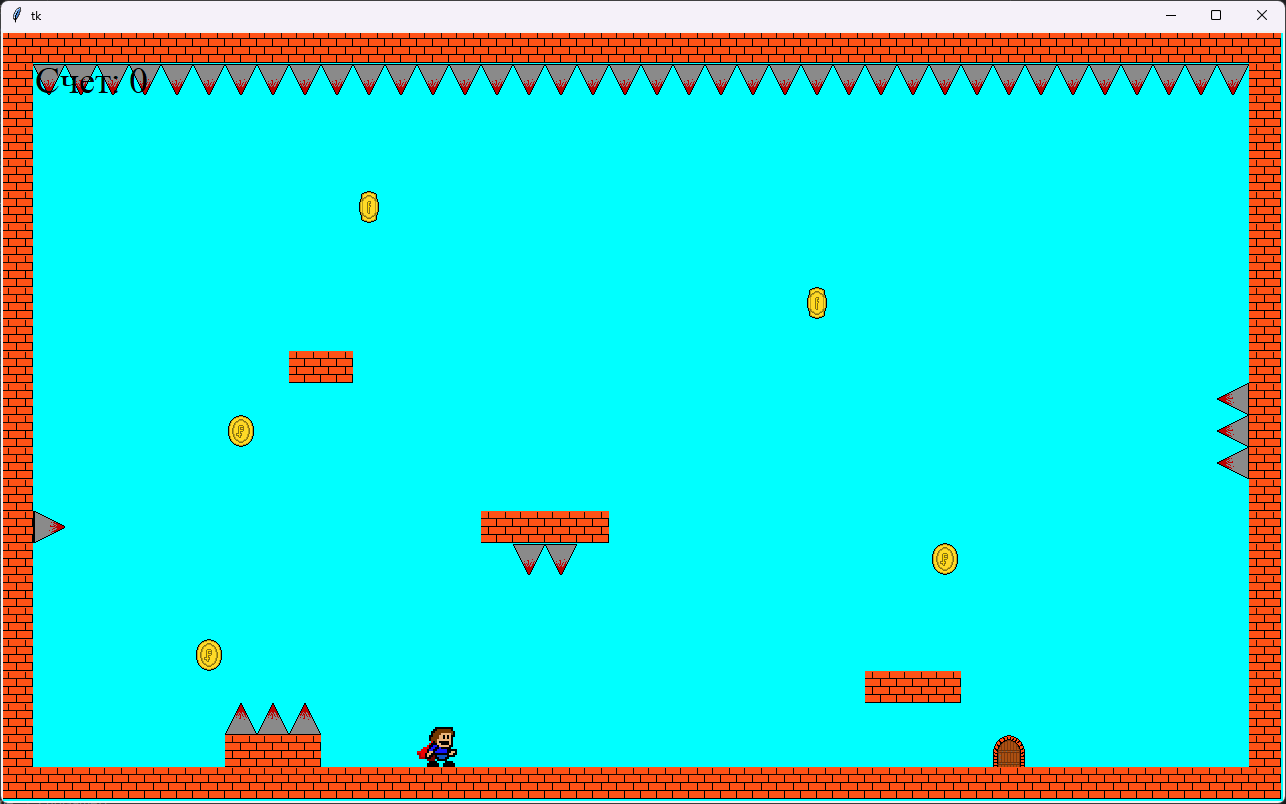
\includegraphics[width=1\linewidth]{main}}
\caption{Главное окно игры}
\label{main:image}
\end{figure}

На рисунке \ref{menu:image} игрок собрал несколько монет.

\begin{figure}[ht]
\center{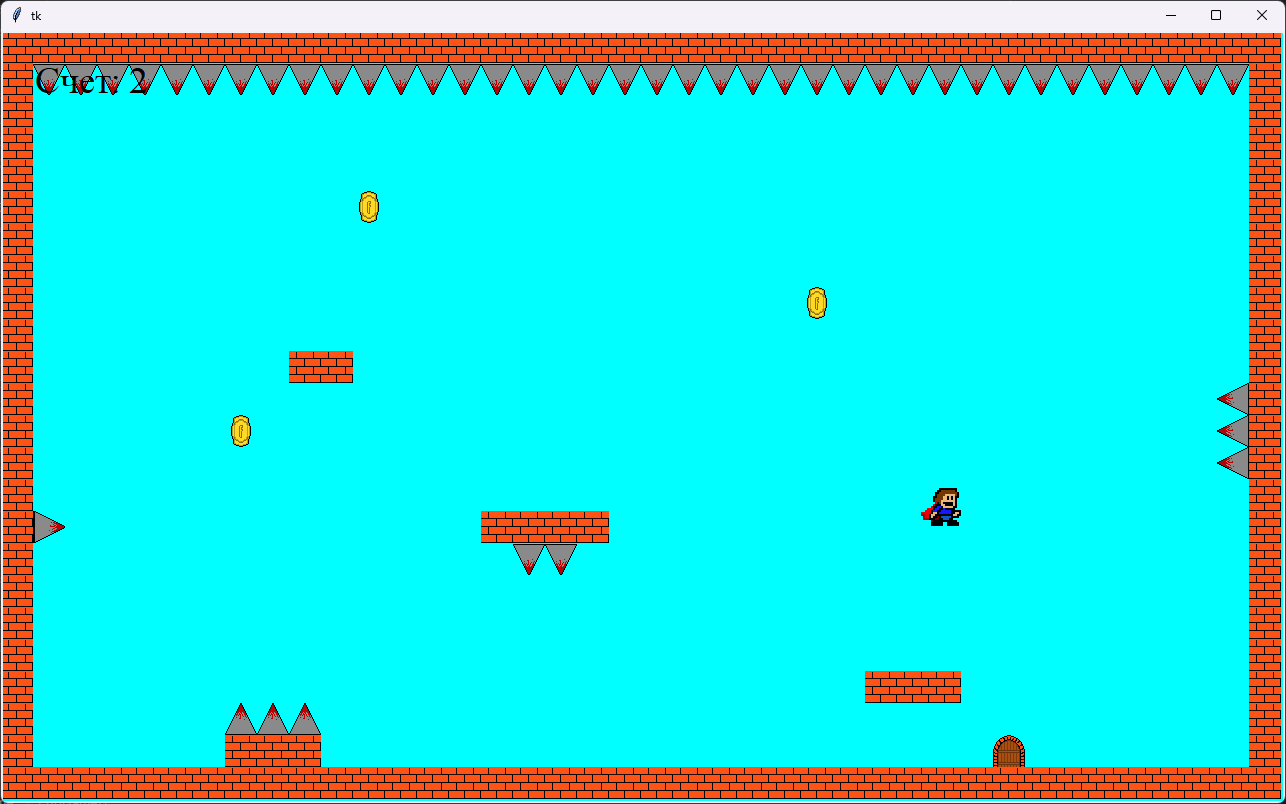
\includegraphics[width=1\linewidth]{menu}}
\caption{Игрок собирает монеты}
\label{menu:image}
\end{figure}

На рисунке \ref{enter:image} игрок собрал все монеты и открыл выход.

\begin{figure}[ht]
\center{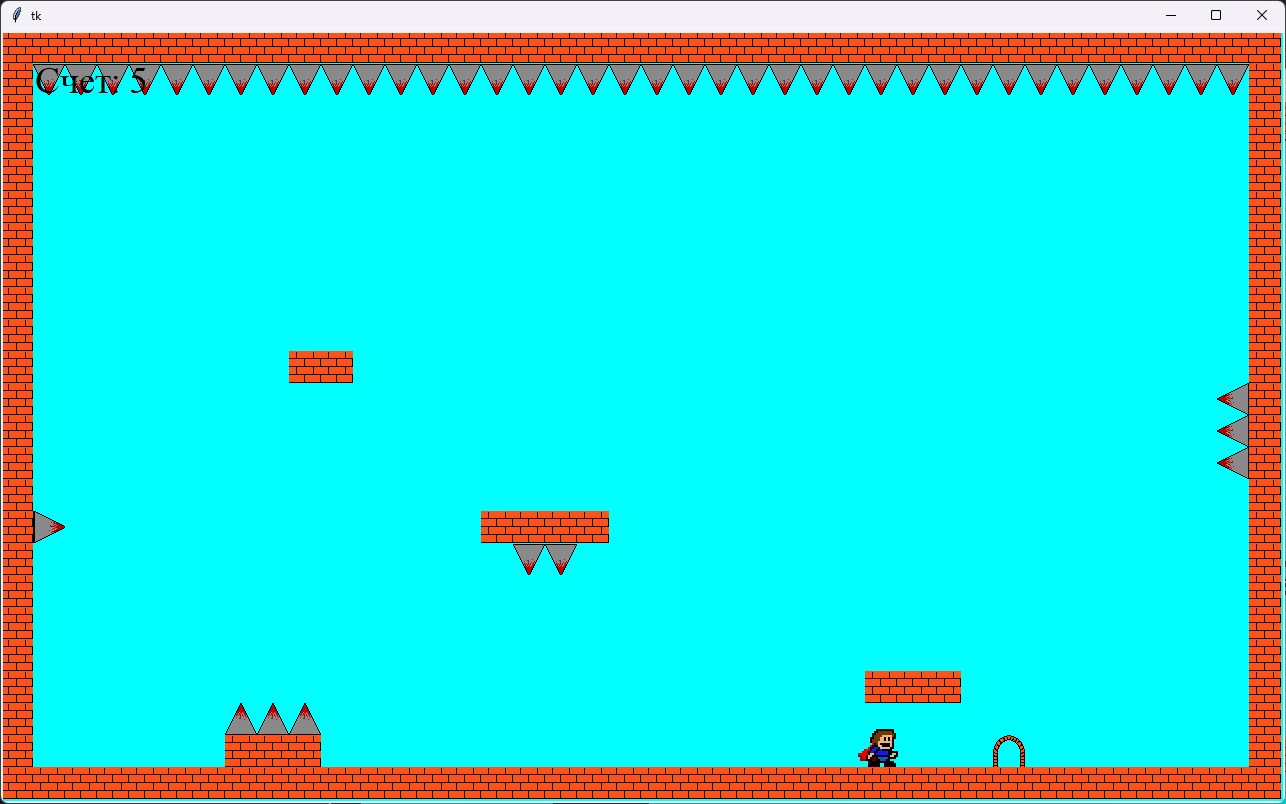
\includegraphics[width=1\linewidth]{enter}}
\caption{Игрок собрал все монеты и открыл выход}
\label{enter:image}
\end{figure}

На рисунке \ref{enter1:image} игрок собрал одну монету и проиграл.

\begin{figure}[ht]
	\center{
\includegraphics[width=1\linewidth]{enter1}}
	\caption{Игрок собрал одну монету и проиграл}
	\label{enter1:image}
\end{figure}

На рисунке \ref{enter2:image} игрок проиграл не собрав ни одной монеты.

\begin{figure}[ht]
	\center{
\includegraphics[width=1\linewidth]{enter2}}
	\caption{Игрок проиграл}
	\label{enter2:image}
\end{figure}

На рисунке \ref{enter3:image} игрок собрал все монеты и добрался до выхода.

\begin{figure}[ht]
	\center{
\includegraphics[width=1\linewidth]{enter3}}
	\caption{Игрок собрал все монеты и покинул уровень}
	\label{enter3:image}
\end{figure}
   \section*{ЗАКЛЮЧЕНИЕ}
\addcontentsline{toc}{section}{ЗАКЛЮЧЕНИЕ}

В ходе выполнения данной курсовой работы была проведена обширная аналитическая работа по изучению особенностей и требований к созданию 2D игр в жанре платформер. Анализ существующих игр этого типа позволил выявить ключевые элементы дизайна, управления, и геймплея, способствующие успешному опыту игрока.

Процесс разработки включал в себя выбор оптимальных инструментов и технологий, а также учет потребностей целевой аудитории.

Реализация проекта демонстрирует успешное внедрение основных принципов, таких как геймплей и интуитивное управление. 

Таким образом, курсовая работа не только раскрывает основные аспекты разработки 2D платформеров, но и предоставляет функциональный пример, демонстрирующий успешное применение теоретических знаний на практике. Полученный опыт может быть полезен для разработчиков, стремящихся создать увлекательные и качественные 2D игры в жанре платформер.

Основные результаты работы:

\begin{enumerate}
\item Проведен анализ предметной области.
\item Проведен обширный анализ существующих 2D игр в жанре платформер.
\item Разработан прототип 2D платформера с учетом современных тенденций.
\item Реализованы основные принципы 2D платформеров.
\end{enumerate}

Все требования, объявленные в техническом задании, были полностью реализованы, все задачи, поставленные в начале разработки проекта, были также решены.
}\fi
\addcontentsline{toc}{section}{СПИСОК ИСПОЛЬЗОВАННЫХ ИСТОЧНИКОВ}

\begin{thebibliography}{9}

    \bibitem{python} Лутц, М. Изучаем Python. Программирование игр, веб-приложений и науки о данных / М. Лутц. – Москва : ДМК Пресс, 2019. – 1280 с. – ISBN 978-5-97060-704-9. – Текст~: непосредственный.
    \bibitem{python} Злобин, С. Программирование игр на Python 3 и Pygame / С. Злобин. – Москва : ДМК Пресс, 2018. – 256 с. – ISBN 978-5-97060-635-6. – Текст~: непосредственный.
    \bibitem{python} Макгроу-Хилл, Э. Python. Эффективное программирование / Э. Макгроу-Хилл. – Санкт-Петербург : Питер, 2018. – 464 с. – ISBN 978-5-496-02911-8. – Текст~: непосредственный.
    \bibitem{python}	Аллен Б. Дауни, Крис Мэйер. Python. Тестирование и разработка / А. Б. Дауни, К. Мэйер. – Санкт-Петербург : Питер, 2020. – 704 с. – ISBN 978-5-4461-1387-3. – Текст~: непосредственный.
	\bibitem{python}	Кэрол А. Грэм. Python. Самоучитель нового поколения / К. А. Грэм. – Москва : Вильямс, 2020. – 480 с. – ISBN 978-5-8459-2146-3. – Текст~: непосредственный.
	\bibitem{python}	Билл Любанович. Python. Тестирование программ. Подробное руководство / Б. Любанович. – Санкт-Петербург : Питер, 2018. – 656 с. – ISBN 978-5-4461-0958-6. – Текст~: непосредственный.
	\bibitem{python}	Аллен Дауни, Эрик Фриман. Python. Программирование на каждый день / А. Дауни, Э. Фриман. – Санкт-Петербург : Питер, 2020. – 528 с. – ISBN 978-5-4461-1352-1. – Текст~: непосредственный.
	\bibitem{python}	Лиза Рассел. Python для детей. Занимательное введение в программирование / Л. Рассел. – Санкт-Петербург : Питер, 2018. – 352 с. – ISBN 978-5-496-03159-3. – Текст~: непосредственный. 
	\bibitem{python}	Лутц, М. Python. Карманный справочник / М. Лутц. – Санкт-Петербург : Питер, 2018. – 416 с. – ISBN 978-5-4461-0926-5. – Текст~: непосредственный.
	\bibitem{python}	Седжвик, Р. Python. Подробное руководство / Р. Седжвик. – Москва : Вильямс, 2017. – 1680 с. – ISBN 978-5-9909015-8-8. – Текст~: непосредственный.
\end{thebibliography}

\ifВКР{\appendix{Представление графического материала}

Графический материал, выполненный на отдельных листах,
изображен на рисунках А.1--А.\arabic{числоПлакатов}.
\setcounter{числоПлакатов}{0}

\renewcommand{\thefigure}{А.\arabic{figure}} % шаблон номера для плакатов

\begin{landscape}

\begin{плакат}
    
\includegraphics[width=0.82\linewidth]{плакат1.png}
    \заголовок{Сведения о ВКРБ}
    \label{pl1:image}      
\end{плакат}

\begin{плакат}
    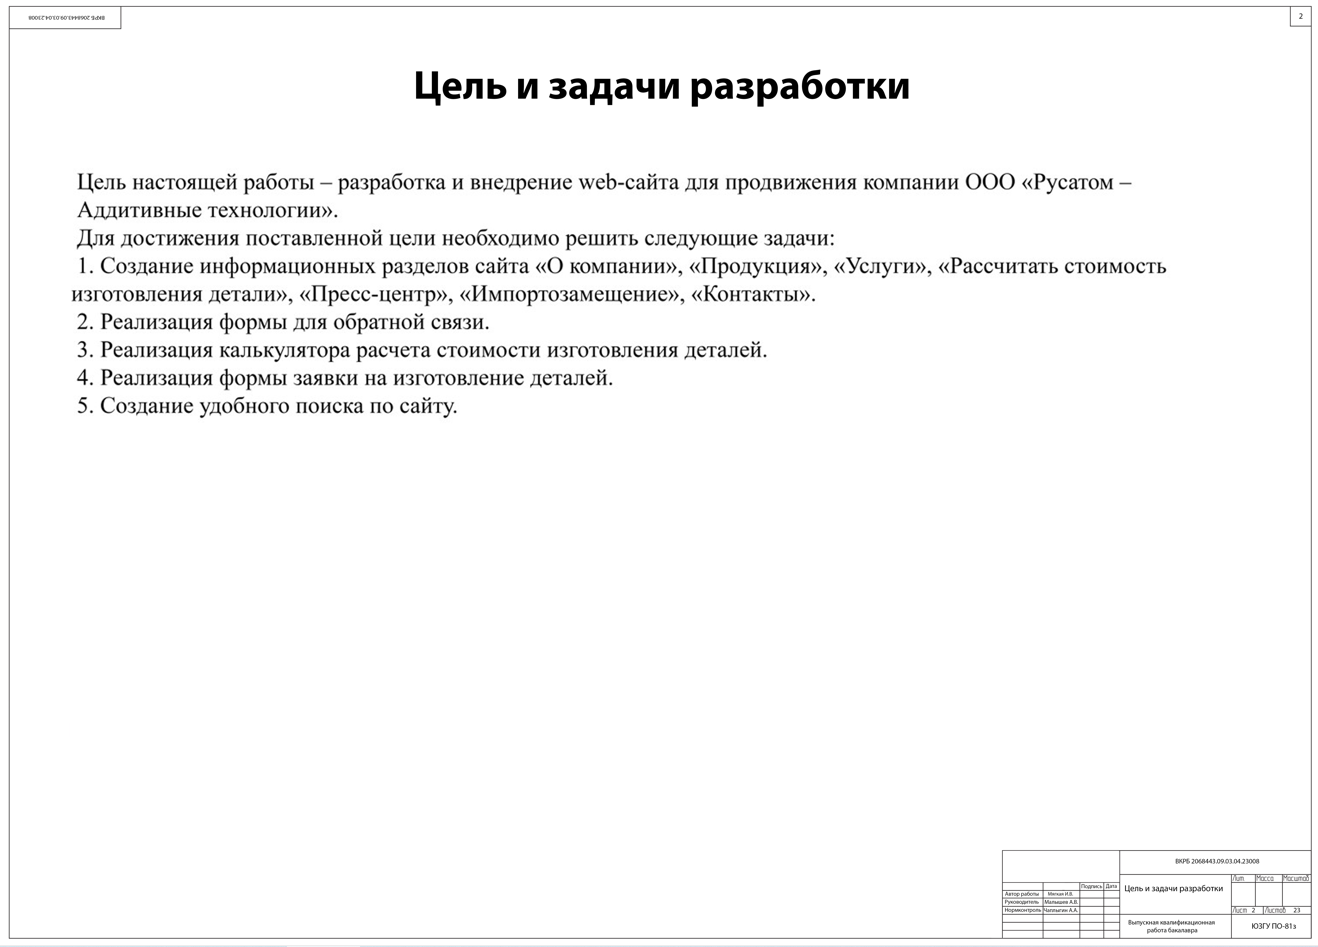
\includegraphics[width=0.82\linewidth]{плакат2.png}
    \заголовок{Цель и задачи разработки}
    \label{pl2:image}      
\end{плакат}

\begin{плакат}
    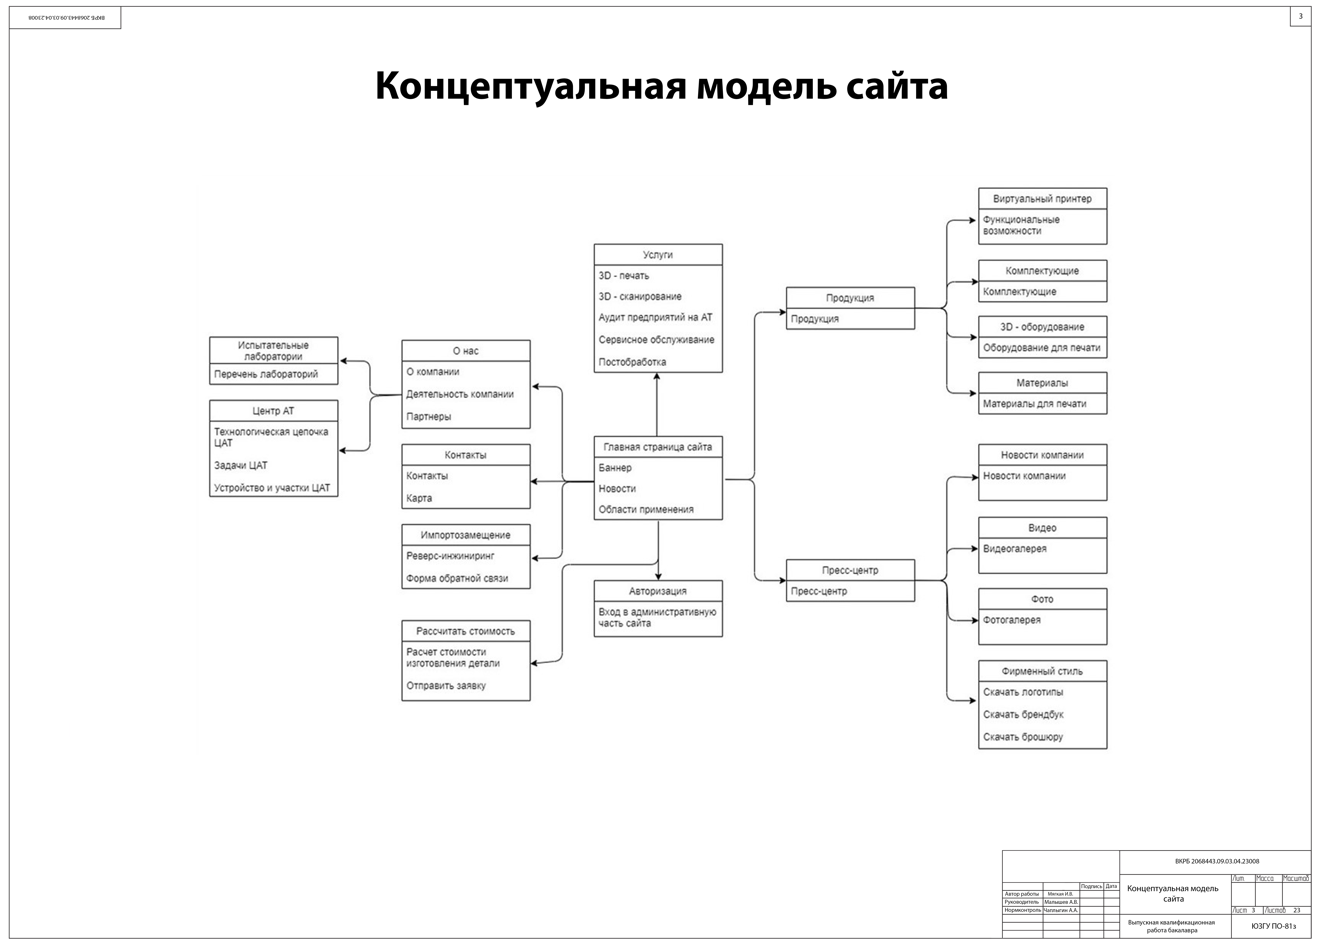
\includegraphics[width=0.82\linewidth]{плакат3.png}
    \заголовок{Концептуальная модель сайта}
    \label{pl3:image}      
\end{плакат}

\begin{плакат}
    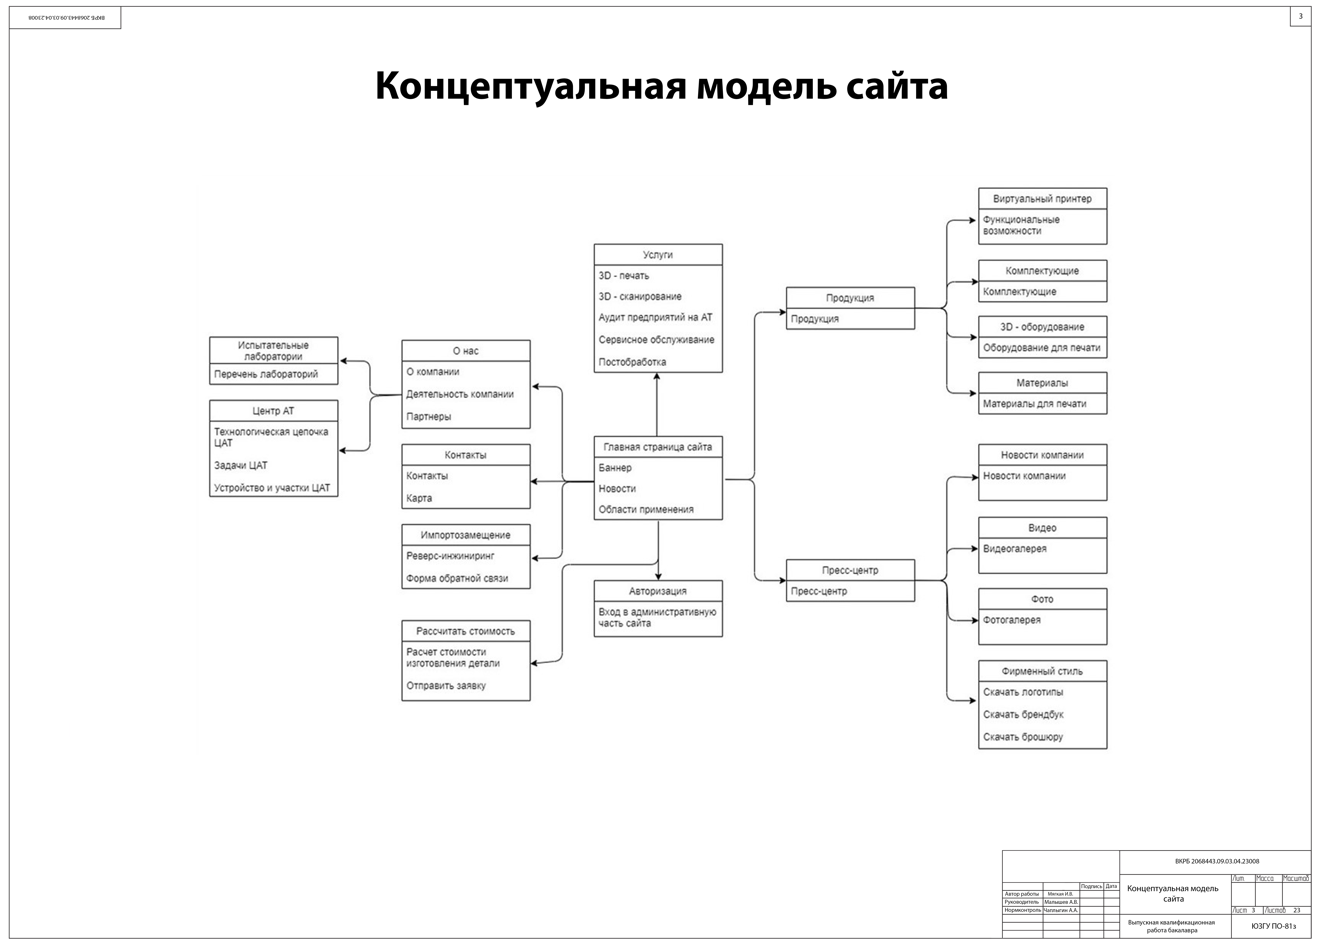
\includegraphics[width=0.82\linewidth]{плакат3.png}
    \заголовок{Еще плакат}
    \label{pl4:image}      
\end{плакат}

\end{landscape}
}\fi
\ifПрактика{}\else{\appendix{Фрагменты исходного кода программы}

main.tex
\lstinputlisting[language=Tex, frame=none]{main.tex}

ТехПроект.tex
\lstinputlisting[language=Tex, frame=none]{ТехПроект.tex}

\ifВКР{
\newpage
\addcontentsline{toc}{section}{На отдельных листах (CD-RW в прикрепленном конверте)}
\begin{center}
\textbf{Место для диска}
\end{center}
}\fi
}\fi
\end{document}
